\section{Correction using timing beacon}
This is to show that the high jitter beacon with poor detection efficiency is already enough to correct for all clock drifts including the change of the Doppler shift for high elevation angles.

\begin{figure}[ht!]
	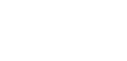
\includegraphics[width=\linewidth]{assets/beacon}
	\caption{The time-stamping units and beacon generator use the same clock reference.}
	\label{fig:beacon}
\end{figure}

